\asection{Background}{Tomáš Sláma}\label{sec:background}

Generative modelling is a subset of the field of machine learning that aims to model an underlying probability distribution of arbitrary data in order to generate new samples that exhibit similar characteristics.

\asubsection{Definitions}{Tomáš Sláma}

For our purposes, we assume there exists a true probability $p^*(X)$, for which we want to find a good approximation $\hat{p}(X)$ using a training set $\left\{X_i \sim p^*(X)\right\}_{i=1}^n$ of true values.

There are two main parts of generative modelling we are interested in:

\begin{enumerate}
    \item \textbf{generation} -- create $X_i$ by sampling $p(X_i)$ \hfill \textit{Get a new sample.}
    \item \textbf{inference} -- calculate $p(X_i)$ for given $X_i$ \hfill \textit{How likely is this sample?}
\end{enumerate}

Since $p^*(X)$ is usually complicated, the most commonly used approach is to introduce a new "code" variable $Z$ and a deterministic function $f$ (which will be learned), such that $Z = f(X)$ and the code probability distribution $q(Z)$ is simple, e.g. Gaussian.

While this works for data and code distribution of the same dimension, this quickly becomes impractical for higer-dimension data (images, sensor data, etc.).
It makes more sense to think of the generative process as "compression/decompression", in which case we define encoder $E: \mathbb{R}^{|X|} \mapsto \mathbb{R}^{|Z|}$ and decoder $D: \mathbb{R}^{|Z|} \mapsto \mathbb{R}^{|X|}$.

Given these definitions, we can describe the properties that we want the models to have, the most important of which are the following:

\begin{enumerate}
    \item \textbf{small codes} -- $\dim(Z) \ll n < \dim{X}$
    \item \textbf{accurate distribution} -- $\hat{p}(X) \approx p^*(X)$
    \item \textbf{good reconstruction} -- $\hat{X} = D(E(X)) \approx X$
\end{enumerate}

\asubsection{Methods}{Tomáš Sláma}

The most popular approaches for generative modelling are outlined in Table \ref{table:gnn-methods}, along with their performance in each of the properties, and are further discussed in the following section.


\begin{table}[ht]
\centering
\begin{tabular}{@{}llll@{}}
\toprule
\multicolumn{1}{c}{\textbf{Goals}}                                                               & \multicolumn{1}{c}{\textbf{VAE} \cite{kingma2013vae}} & \multicolumn{1}{c}{\textbf{GAN} \cite{goodfellow2014gan}} & \multicolumn{1}{c}{\textbf{NF} \cite{rezende2016nf}} \\ \midrule
\textbf{small codes}                                                                             & hyperp.                          & hyperp.                          & bad (lossless)                        \\
\textbf{accurate distribution}     & trade-off                        & good                             & good                            \\
\textbf{good reconstruction} & trade-off                        & N/A                            & good                            \\
\textbf{has inference} & no                        & no                            & yes                            \\\bottomrule
\end{tabular}
\caption{A summary of methods for generative modelling using neural networks.}\label{table:gnn-methods}
\end{table}

\textbf{Variational Auto-Encoders} (\textbf{VAE}s) \cite{kingma2013vae} replace deterministic functions $f(X)$ and $q(Z)$ with conditional distributions $p_E(X \mid Z)$ and $p_D(X \mid Z)$. Both are then trained jointly using $\mathrm{ELBO}$ loss, which balances the distribution accuracy and the reconstruction error.
Most commonly, the decoder and encoder are diagonal Gaussians since these are numerically tractable.

\textbf{Generative Adversarial Networks} (\textbf{GAN}s) \cite{goodfellow2014gan} train two models simultaneously: a generative model ($G$) that generates data samples, and a discriminative model ($D$) that distinguishes between real and generated samples.
$G$ is trained to maximize the likelihood of $D$ making errors and, analogously, $D$ is trained to minimize those errors. In practice, both $D$ and $E$ are neural networks.

\textbf{Normalizing Flows} (\textbf{NF}s) \cite{rezende2016nf} define methods for transforming a simple code distribution $q(Z)$ into a more complex distribution through a series of invertible and differentiable mappings. 
This allows for the evaluation of the density of a sample (something not possible for VAEs and GANs) and therefore supports both generation and inference.


\asubsection{Normalizing Flows and Beyond}{Tomáš Sláma}\label{sec:nf_explanation}

Since Normalizing Flows form the basis for SurVAE and are therefore relevant for the rest of the paper, we will cover them here in greater detail.

As the brief summary above suggests, the goal is to take a simple distribution (usually the standard normal, hence \textit{normalizing} flows) and transform it into a more complex one by a series of bijective transformations.
This is based on the multi-dimensional change-of-variables formula -- given two densities $q(Z), p(X)$ and an invertible function $f$ such that $f(X) = Z$, the following holds true: \begin{equation}
 p(X) = q(f(X)) \cdot | \det \mathcal{J}_f (X) |   
\end{equation}\label{eq:p-bij}%
Setting $q(Z) = \mathcal{N}(0, 1)$ as our simple distribution to transform, we want to obtain $f$ (=train, since we will use a neural network for this task).

To be able to do this efficiently (and, at all actually), we have to make sure that $f$ is computable, invertible and that $\det \mathcal{J}_f (X)$ can be calculated efficiently.
Since we have freedom in the choice of the architecture, we can choose to make the layers autoregressive, making their determinants triangular and therefore easy to calculate.

A common architecture is to change only half of the dimensions (with the others being skip connections) -- given the $(l-1)$-th layer (denoted $Z^{(l-1)}$) of dimension $D$, we calculate the $(l)$-th layer in the following way:

\[\begin{aligned}
	Z_{j}^{(l)} &= Z_{j}^{(l-1)} \; &&\forall j=1, \ldots, \tilde D \quad \text{for}\ \tilde D = \left\lfloor D/2 \right\rfloor \\ Z_j^{(l)} &= f_j^{(l)} \left(Z_j^{(l-1)}, Z_{1:\tilde D}^{(l-1)}\right) \; &&\forall j = \tilde D + 1, \ldots, D
\end{aligned}\]

making the Jacobian triangular:

\[\mathcal{J}^{(l)} = \begin{pmatrix}
  \mathrm{I}_{\tilde D} & \mathrm{0}_{\tilde D} \\
  \neq 0 & \mathrm{diag}\left(\frac{\partial f_j^{(l)}}{ \partial Z_j^{(l-1)}}\right) \\
\end{pmatrix}\]

A popular choice for $f$ is affine, i.e. \(Z_{j}^{(l)} = s \cdot Z_j^{(l-1)} + t\) (for $s \neq 0$), which is also the one used by us.

Since just placing these layers (referred to from now on as bijective, see \ref{sec:bijective}) will skip the first half of the input, they are combined with orthonormal layers (see \ref{sec:orthonormal}) to transform the distribution using an orthonormal transformation.

With this in mind, the subject of this paper, \textbf{Surjective Variational Auto-Encoders} (\textbf{SurVAE}s), aim to extend the possible transformations from bijective to stochastic by using the fact that we can approximate any density via the following equation (Eq. 2 in the original paper): $$\log p(X) \simeq \log p(Z) + \mathcal{V}(Z) + \mathcal{E}(X, Z)$$
for $\mathcal{V}$ likelihood contribution and $\mathcal{E}$ bound looseness.
We have already seen that $\mathcal{V}(Z) = \log |\det \mathcal{J}|$ (Eq. \ref{eq:bijective}), and we can calculate that $\mathcal{V}(Z) = \log \frac{p(X \mid Z)}{p(Z \mid X)}$ for stochastic ones (with some non-zero looseness), which is all we need for using both kinds of layers.

\subsection{Data}

\textit{Note that we always use the color range ``viridis", which is the standard of the python library \texttt{matplotlib}, instead of black-to-white, which would at times be more appropriate.}


\asubsubsection{Synthetic Data}{Tomáš Sláma}

\textit{The results are taken from the \href{https://github.com/xiaoxiae/GNNFinal2024/blob/main/notebooks/datasets.ipynb}{notebooks/datasets.ipynb} notebook.}

There are a number of synthetic datasets that we use throughout the experiments, each of which contains certain attributes we want to test the network on, which includes (but is not limited to) symmetry, anti-symmetry, discontinuities and precise/fuzzy borders.
They can be either unlabeled or labeled, both of which are described in Figures \ref{fig:synt-nolab} and \ref{fig:synt-lab} respectively.

\begin{figure}
{\centering%
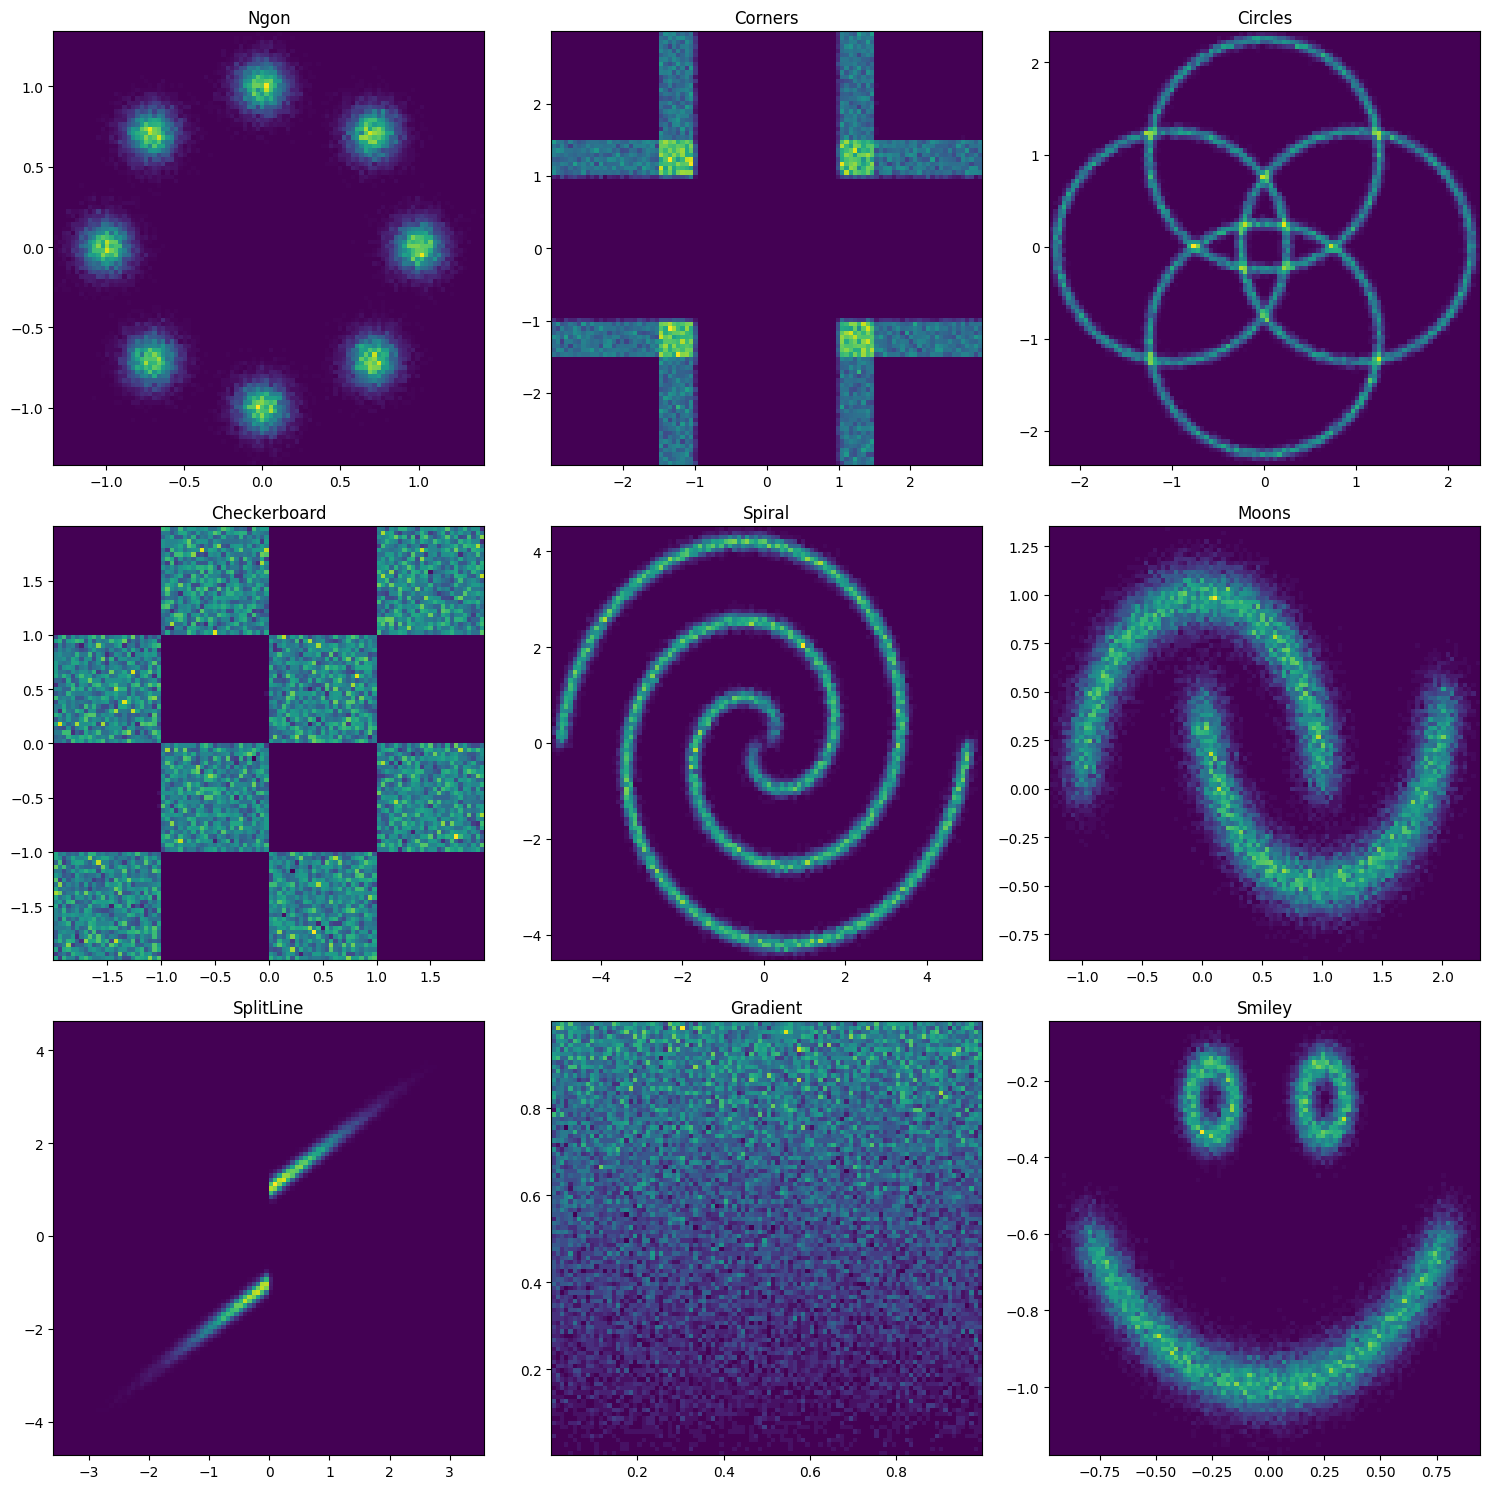
\includegraphics[width=\textwidth]{images/synthetic/overview/synt-nolab.png}
\caption{Synthetic unlabeled datasets ($10\,000$ samples each).}\label{fig:synt-nolab}}

\vspace{2em}

\dataset{Ngon} $n$ Gaussians with constant noise arranged along a circle.

\dataset{Corners} $4$ disjoint corners with overlaps (with doubled density).

\dataset{Circles} $n$ circles with equal radius arranged along a circle.

\dataset{Checkedboard} a tiling of size $n^2$, sampling only one tile color.

\dataset{Spiral} a double spiral, symmetric around the origin.

\dataset{Moons} the standard two moons dataset.

\dataset{SplitLine} A thin Gaussian separated by an offset in the middle.

\dataset{Gradient} Essentially noise -- randomly sample $x$, $x^2$ and concatenate.

\dataset{Smiley} a combination of two circles and a semi-circle.
\end{figure}

\begin{figure}
\centering
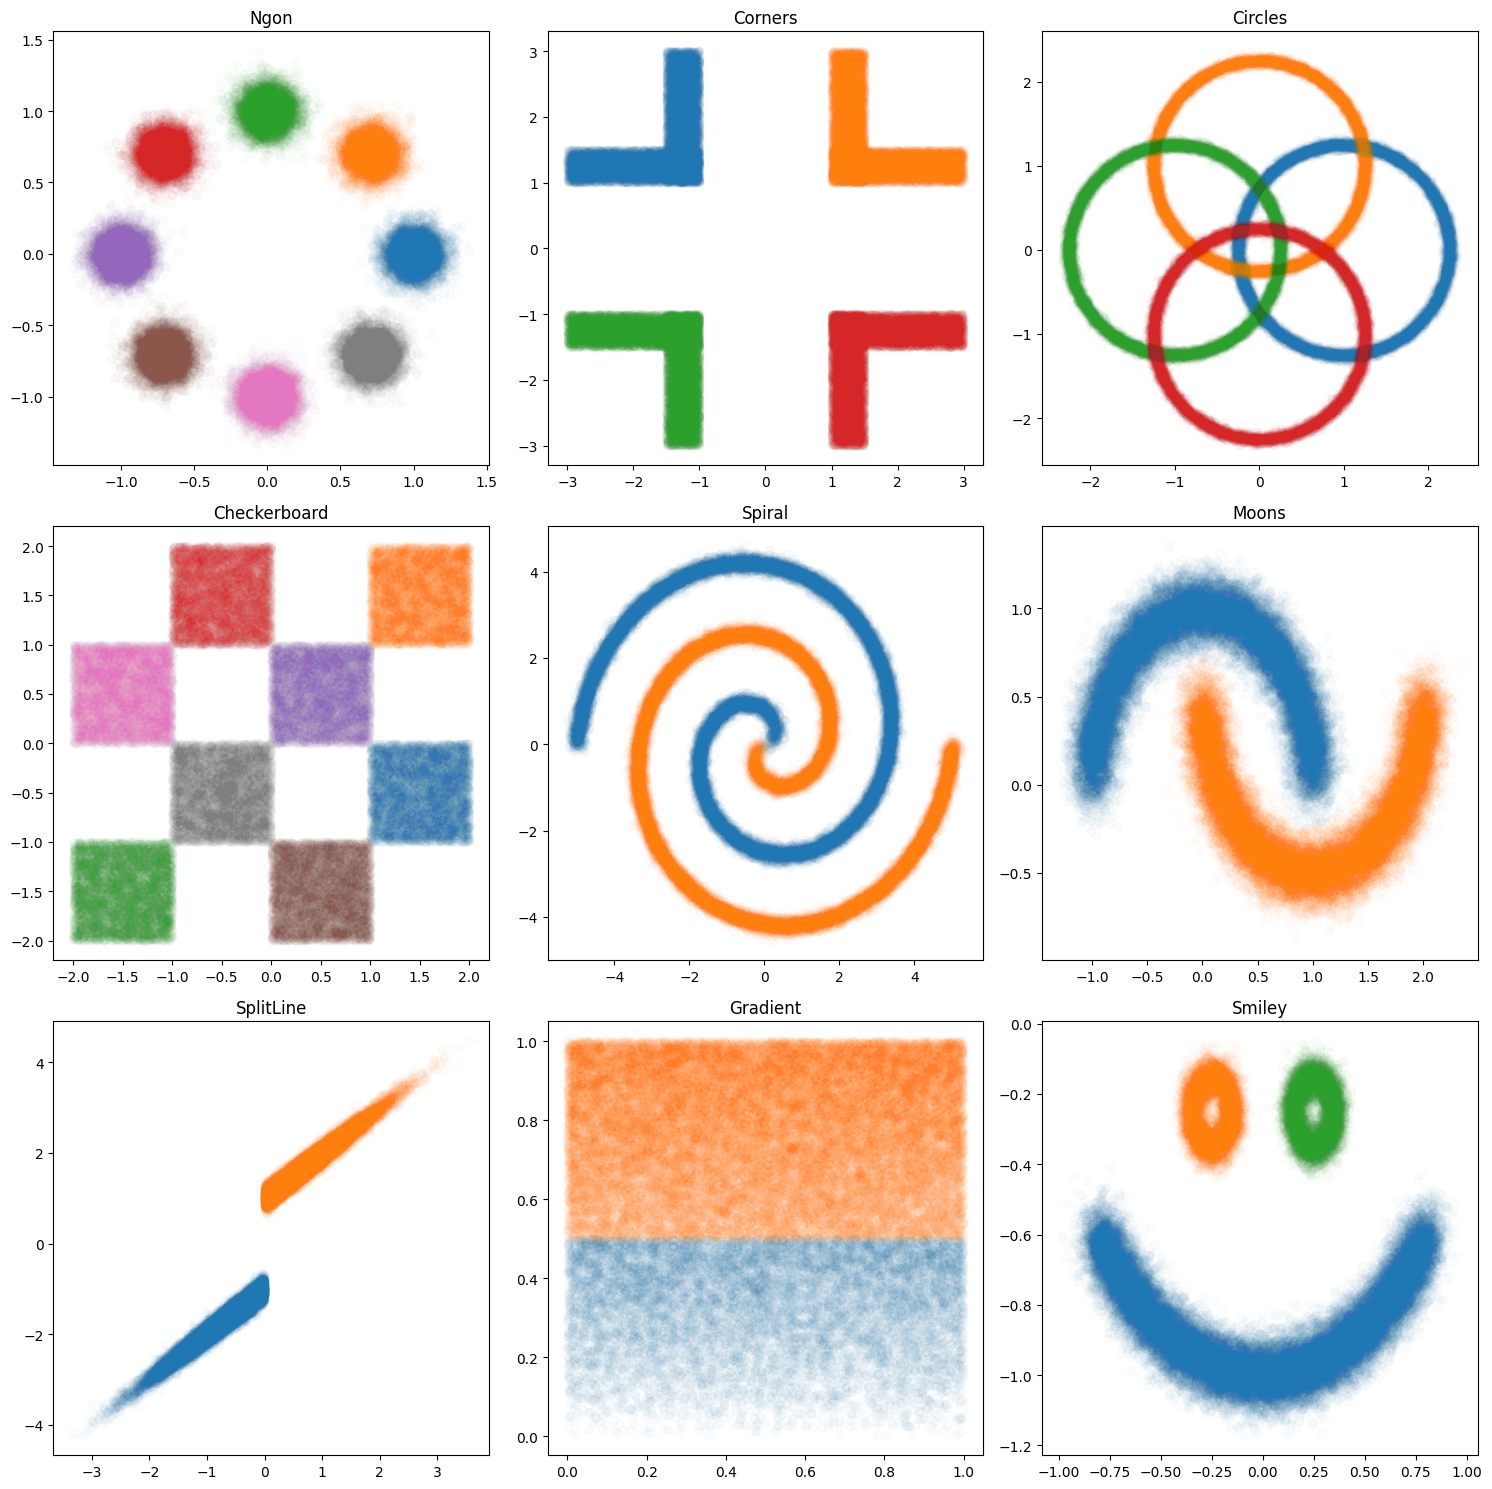
\includegraphics[width=\textwidth]{images/synthetic/overview/synt-lab.png}
\caption{Synthetic labeled datasets ($10\,000$ samples each). The categories were picked in the most intuitive way, also making sure that each dataset has $ \geq 2$.}\label{fig:synt-lab}
\end{figure}

\begin{figure}
\centering
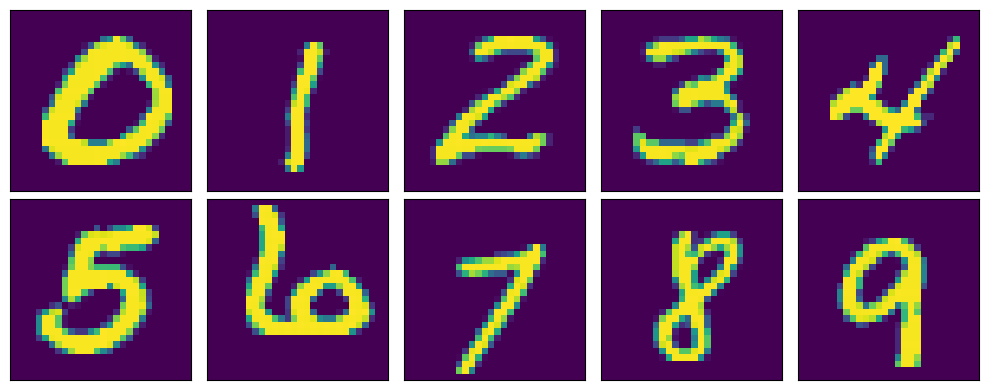
\includegraphics[width=\textwidth]{images/mnist_maxpooling/mnist_dataset.png}
\caption{Example images from the MNIST784 dataset.}
\label{fig:mnist784_example}
\end{figure}


\asubsubsection{Image Data}{Jannis Heising}
As reasoned in Section~\ref{sec:image_data}, we used the MNIST784 dataset for our image data experiments as opposed to the more complex sets used in~\cite{nielsen2020survae}. MNIST784 consists of 70,000 grey-scale images, each of size 28x28 and displaying one of the ten digits 0-9, as shown in Figure~\ref{fig:mnist784_example}.


\asubsubsection{Point Cloud Data}{Maria Stickel}

Similar to \cite{nielsen2020survae} and \cite{edwards2017neural}, we wanted to train our model on the spatial MNIST data set, where instead of directly using the images of hand-written digits, one uses the probability weights over the images of the hand-written digits to sample coordinates for single points which together as a cloud represent the digit.

In general, one input vector to the network describes a single point sampled from the underlying distribution. In the synthetic datasets, this is a single point from a two-dimensional vector space, drawn from the underlying distribution. In the case of the point cloud data, a single input point is a cloud of points and therefore contains several point samples from the distribution of weights over the image. This resulted in quite some issues when applying the previously easy-to-use modular framework of layers, where we saw very good results pretty fast.

Our initial approach on how to handle the points was pretty much "flatten everything" and "unflatten if necessary". An example of this is be the \texttt{MaxPoolingLayer} (\ref{sec:max_pooling_layer}) operation for the previously described plain MNIST dataset. For the spatial MNIST data, operations like permutations break the structure of the array in the sense as it would not permute the sampled points as tuples, but also permute points and their x- and y-coordinates, removing the possibility for the model to understand the underlying dependencies of the coordinates. Therefore we introduced layers that don't appear in \cite{nielsen2020survae}: \texttt{PermuteAxesLayer} (\ref{sec:permute_axes_layer}) and \texttt{ReshapeLayer} (\ref{sec:reshape_layer}) to address this issue. We also modified the \texttt{BijectiveLayer} to operate on this type of structured data, which was a changing point for the results (see \ref{sec:spatial_mnist}).

Both referenced papers used 50 points to represent a digit, and in our final experiments we followed their approach. Initially, we also experimented with a smaller number of points, 30 to be exact, as we were curious to see whether this is sufficient, but the results were worse. We dropped that and don't include it here. 

\asubsubsection{SIR Data}{Jannis Heising}\label{sec:sir_data}
The SIR model aims to describe how an infectious disease spreads throughout a population. The population $N$ is spread into three \textit{compartments}, namely Susceptible $S$, Infectious $I$, and Removed $R$. For simplicity, the population size is normalized to 1, meaning that the values $S$, $I$, and $R$ represent the \textit{fraction} of the population belonging to that compartment.

Given these fractions, the SIR model prescribes their rate of change as an ordinary differential equation (ODE):
\begin{align*}
    \frac{\dd S}{\dd t} &= -\lambda \cdot S \cdot I,\\
    \frac{\dd I}{\dd t} &= \lambda \cdot S \cdot I - \mu \cdot I,\\
    \frac{\dd R}{\dd t} &= \mu \cdot I.
\end{align*}

Here, $\lambda$ and $\mu$ are parameters that determine the behaviour of the system. The other parameters are the \textit{initial values} $S_0$, $I_0$, and $R_0$ of the fractions at time {$t = 0$}. To simplify the model, we always set {$S_0 = R_0 = 0$}. Thus, the system behaviour is completely determined by the three parameters $\lambda$, $\mu$, and $I_0$.

In the setting of SBI, these three values are the \textit{hidden parameters}. A simulation then produces their corresponding \textit{observational data}. We use a simple Euler-forward method with step size 0.1 to simulate the ODE above for 100 days (i.e. until {$t = 100$}). The data then consists of the rate-of-change values $\frac{\dd S}{\dd t}$ and $\frac{\dd R}{\dd t}$ at each step.

\asubsection{Parameter Degeneracy and SBI}{Jannis Heising}\label{sec:background_param_degen}

One of our experiments revolves around parameter degeneracy of simulation-based inference (SBI), thus we briefly introduce those terms.

\textbf{Simulation-based Inference (SBI)} is a method for identifying hidden parameters of observational data with the help of an existing simulation. A prime example is understanding the spread of a disease when given infection rate data on one hand and a theoretical framework in the form of a simulation on the other. The simulation takes the hidden parameters and turns them into observation-like data, so SBI can be thought of as an inverse to the simulation.

In practical terms, the setup for SBI is as follows: Let $\{Y_k^{*}\}_{k=1}^K$ be $K$ sets of hidden parameters and $\{X_k = \Phi(Y_k^{*})\}_{k=1}^K$ their respective outputs of the simulation $\Phi$. We then train a conditional NF on the dataset $\{(Y_k; X_k)\}_{k=1}^K$, i.e. we train it to generate the parameters $Y_k$ given the condition $X_k$.

\textbf{Parameter degeneracy}, in the context of this report, is a shortcoming of normalizing flows which occurs when the data manifold does not have the same dimension as the latent space. For example, if one were to train a two-dimensional NF on points lying solely on a one-dimensional shape like a circle embedded in two-dimensional euclidean space, one would be presented with an underwhelming result (see Section~\ref{sec:simple_degen}).

In the lecture, we briefly touched on parameter degeneracy in the context of SBI: It may happen that not all hidden parameters can be unequivocally recovered from the observed data. As an example, we chose the most basic SIR model (see Section~\ref{sec:sir_data}). Note that the article uses $\beta$ and $\gamma$ instead of $\mu$ and $\lambda$. with only three parameters $\mu$, $\lambda$, and $I_0$ and made it degenerate by replacing $\lambda$ with two new parameters $\lambda_1$ and $\lambda_2$. For the simulation, these values are multiplied to end up with only one value $\lambda = \lambda_1 \cdot \lambda_2$, thus the original two values cannot be recovered from the simulation output alone.
